\section{Definite integral}


\paragraph{What is area?}
Properties of area:
\begin{enumerate}
	\item For a rectangle $S=ab$
	\item For disjoint $S_1$, $S_2$, $Area(S_1 \cup S_2) = Area(S_1)+Area(S_2)$
	\item If $S_1 \subseteq S_2$ then $Area(S_1) \leq Area(S_2)$.
\end{enumerate}

\paragraph{Area under the function}

\begin{center}
	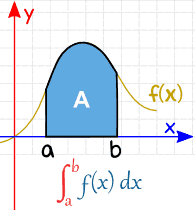
\includegraphics{./lect1/pic1.png}
\end{center}
$$f:[a,b] \to R$$
$$m \leq f(x) \leq M \quad \forall a \leq x \leq b$$
It's obvious that $m(b-a) \leq S\leq M(b-a)$. Define partition $P$ of $[a,b]$:
$$a=x_0<x_1<\dots<x_n=b$$
Given partition $P$ denote 
$$m_i := \inf f(x) [x_{i-1} x_{i}]$$

$$M_i := \sup f(x) [x_{i-1} x_{i}]$$
$$\Delta x_i = x_i - x_{i-1}$$

\begin{center}
	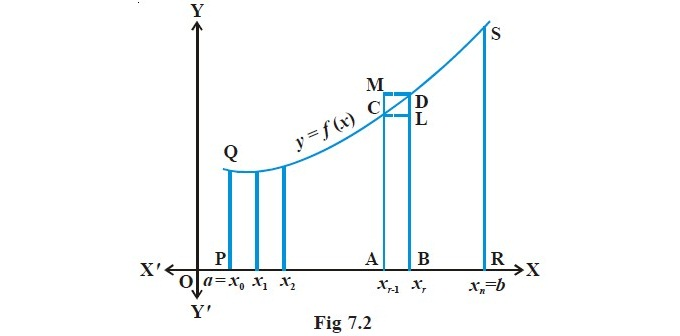
\includegraphics{./lect1/pic2.jpg}
\end{center}
For each of intervals $[x_{i-1}, x_i]$ the area under the graph is $m_i\Delta x_i \leq S_i \leq M_i \Delta x_i$. Then for the total area, due to property 2, we want
$$\sum_{i=1}^n m_i \Delta x_i \leq S \leq \sum_{i=1}^n M-i \Delta x_i$$

Denote:
$$U(P,f) = \sum_{i=1}^n M_i \Delta x_i$$
$$L(P,F) = \sum_{i=1}^n m_i \Delta x_i$$
which are called upper and lower Darboux sums.
$$\forall P \quad L(P,f) \leq S \leq U(P,f)$$

\paragraph{Refinements} Let $P$, $P^\prime$ two partitions of $[a,b]$. $P^\prime$ refines $P$ if each point in $P$ is also in $P^\prime$. 
\paragraph{Claim} $U(P^\prime) \leq U(P)$ and $L(P^\prime) \geq L(P)$.
\subparagraph{Proof} 
$$P:\: a=x_0<x_1<\dots<x_n=b$$
$$P^\prime:\: a=x_0<x_1<\dots x_k<x^\prime < x_{k+1}< \dots<x_n=b$$
Denote $M^\prime = \sup f [x_k, x^\prime]$ and $M^{\prime \prime} = \sup f [x^\prime, x_k+1]$.
Then $U(P^\prime) = M_1 \Delta x_1 + \dots + M_K \Delta x_k + M^\prime \left( x^\prime - x_k \right) + M^{\prime \prime} \left( x_{k+1} - x^\prime \right) + \dots$
$$U(P^\prime)-U(P) = M^\prime \left( x^\prime - x_k \right) + M^{\prime \prime} \left( x_{k+1} - x^\prime \right) - M_{k+1} \left( x_{k+1} - x_k \right)$$
But $M^\prime, M^{\prime \prime} \leq M_{k+1}$
$$U(P^\prime)-U(P) \leq M_{k+1} \left(x_{k+1} - x_k\right) -  M_{k+1} \left(x_{k+1} - x_k\right) = 0$$

\paragraph{} Denote parameter of partition $\lambda(P) = \max_i \Delta x_i$
\paragraph{Note} Given two partitions $P, P^\prime$ exists partition $P^{\prime \prime}$ which includes both of them (acquired by union)
\paragraph{Conclusion} For any two partitions $P$, $P^\prime$ $L(P) \leq U(P^\prime)$
\subparagraph{Proof} Let $P^{\prime \prime}$ mutual refinement of $P$ and $P^\prime$. Then
$$L(P) \leq L(P^{\prime \prime}) \leq U(P^{\prime \prime}) \leq U(P^\prime)$$
\paragraph{Conclusion} $\sup L(P) \leq \inf (U(P))$.
\paragraph{Definition} Let $f$ bounded on $[a,b]$. We say that $f$ is Riemann integrable if $\sup L(P) = \inf (U(P))$. In this case we denote this value $\int_a^b f(x) dx$ and call it definite integral of $f$ on $[a,b]$. If this integral exists we can think on it as area under $f$ on $[a,b]$.

When $f(t)$ denotes temp of change then $\int_a^b f(t) dt$ denotes total change.
\subsection{Examples}
\paragraph{} 
$$
D(x) = \begin{cases}
0&x\in\mathbb{Q}\\
1&x\notin\mathbb{Q}\\
\end{cases}
$$
For any partition $L(P,D) = 0$ and $U(P,D) = 1 \Rightarrow$ $D$ isn't integrable.
\paragraph{} $f(x) = c$ on $[a,b]$. Then $M_i = m_i = c$. By definition $$\int_a^b c dx= c(b-a)$$ 
\paragraph{} $f(x) =x$ on [0,1]. Define $P_n: 0 < \frac{1}{n}  < \frac{2}{n} < \dots < \frac{n-1}{n} < 1$. Then
$$U(P_n,f) = \frac{1}{n} \cdot \frac{1}{n} +  \frac{2}{n} \cdot \frac{1}{n} + \dots +  1 \cdot \frac{1}{n} = \frac{1}{n^2} \cdot \sum_{k=1}^{n} k = \frac{1}{n^2} \cdot \frac{n(n+1)}{2}  = \frac{1}{2} \left( 1+ \frac{1}{n} \right)$$ 
Similarly
$$L(P_n,f) = \frac{1}{n^2} \cdot \sum_{k=1}^{n} \left(k-1\right) = \frac{1}{2} \left( 1+- \frac{1}{n} \right)$$ 
Then $\inf U(P_n, f) = \sup L(P_n,f) = \frac{1}{2}$. However, those are not all partitions. But
$$\frac{1}{2} \leq \sup L(P,f) \leq \inf U(P,f) \leq \frac{1}{2}$$
meaning $f(x)$ is integrable and $\int_0^1 x dx =\frac{1}{2}$.
\paragraph{Theorem} Given $P\subseteq P^\prime$, suppose $P^\prime$ is refinement of $P$ acquired by adding $q$ points. Then $0 \leq U(P) - U(P^\prime) \leq \lambda(P)\cdot q \cdot (M-m)$ and $0 \leq L(P^\prime) - L(P) \leq \lambda(P)\cdot q \cdot (M-m)$.
\subparagraph{Proof} With previous symbols, i.e 
$$P:\: a=x_0<x_1<\dots<x_n=b$$
$$P^\prime:\: a=x_0<x_1<\dots x_k<x^\prime < x_{k+1}< \dots<x_n=b$$
$M^\prime = \sup f [x_k, x^\prime]$ and $M^{\prime \prime} = \sup f [x^\prime, x_k+1]$.

Suppose $q=1$ (it's enough), then
\begin{align*}
U(P) - U(P^\prime) = M_{k+1} \underbrace{\left( x_{k+1} - x_k \right)}_{x_{k+1}-x^\prime + x^\prime - x_k} - M^\prime \left( x^\prime - x_k \right) - M^{\prime \prime} \left( x_{k+1} - x^\prime \right) = \left(M_{k+1} - M^\prime\right)\left( x^\prime - x_k \right) +  \left(M_{k+1} - M^{\prime\prime}\right)\left( x_{k+1} - x^\prime \right) \leq\\
\leq (M-m)(x^\prime-x_k)+(M-m)(x_{k+1}-x^\prime) = (M-m)(x^\prime - x_k + x_{k+1}-x^\prime) = (M-m)\Delta x_{k+1} \leq (M-m) \cdot \lambda(P)
\end{align*}
\paragraph{Theorem} Following conditions are equivalent for bounded $f(x)$:
\begin{enumerate}
	\item $f(x)$ is integrable
	\item $\forall \epsilon > 0 \: \exists P_\epsilon$ such that $U(P_\epsilon) - L(P_\epsilon) < \epsilon$. Denote $W(P_\epsilon, f) = U(P_\epsilon) - L(P_\epsilon) = \sum \left(M_i - m_i\right) \cdot \Delta x_i$
	\item $\forall \epsilon > 0 \: \exists \delta > 0 $ such that if $\lambda(P) < \delta$ for some $P$, then $W(P) < \epsilon$.
\end{enumerate}
\subparagraph{Proof} Obviously, $3 \Rightarrow 2$.

If 2 is right, then $\inf U(P) - \sup L(P) \leq U(P_\epsilon) - L(P_\epsilon) < \epsilon \quad \forall \epsilon > )$, i.e. $\inf U(P) - \sup L(P) = 0$.

Now let's proof $1 \Rightarrow 3$. Suppose $f(x)$ is integrable and denote $I = \int_a^b f(x) dx$. Let $\epsilon > 0$ then exists $P^\prime$ such that $I \leq U(P^\prime) \leq I + \frac{\epsilon}{4}$ (since $I$ is infimum). 

Let's choose $\delta = \frac{\epsilon}{4n(M-m)}$ when $n$ is number of points in $P^\prime$. (if $M=m$ then proof is trivial).

We choose $P$ such that $\lambda(P) < \delta$ and $P^{\prime\prime}$ is union of points of $P$ and $P^\prime$. Suppose there are $p$ more points in $P^{\prime\prime}$ than in $P$. Note that $p \leq n$. Then
$$I \leq U(P) \leq U(P^{\prime \prime}) + \lambda(P)\cdot p\cdot(M-m) \leq U(P^{\prime \prime}) + \lambda(P) \cdot n \cdot (M-m) \stackrel{\scriptsize \delta = \frac{\epsilon}{4n(M-m)}}{\leq} U(P^{\prime \prime})  + \frac{\epsilon}{4} \leq U(P^\prime)  + \frac{\epsilon}{4} \leq I + \frac{\epsilon}{2} $$
which means $I \leq U(P) \leq I+\frac{\epsilon}{2}$. Similarly we can get $I \geq L(P) \geq I-\frac{\epsilon}{2}$, i.e. $W(P) < \epsilon$